% INTRODUCCION

\section{Acerca de la tesis de licenciatura}

Durante la tesis de licenciatura se analizaron las variaciones en los parámetros del clima. Los mismos son utilizados en la corrección de los eventos adquiridos por el observatorio Pierre Auger. Estas variaciones son causadas por las distintas condiciones atmosféricas durante el desarrollo de las EAS. Se analizaron los datos adquiridos durante en el periodo 2005-2018 por el arreglo de SDs espaciados 1500 m entre sí, conocido como \emph{arreglo principal}. De esta manera, se extendió los periodos estudiados anteriormente en los siguientes trabajos \cite{abraham2009atmospheric}, \cite{abreu2012description}   y \cite{aab2017impact}. 

También se emuló el análisis de la modulación del clima sobre el periodo 2005-2015 \cite{aab2017impact}, obteniéndose resultados compatibles. Se observó que en los eventos posteriores a la corrección, la modulación del clima se vio disminuida. Esta modulación es despreciable para eventos con energía mayor a $2\,$EeV.

En el mismo trabajo, se estudió la modulación del clima mediante el valor del $S_{38}$ sin la corrección propuesta por trabajos mencionados. Se observó que los parámetros del clima obtenidos en este análisis son compatibles con los utilizados en la reconstrucción oficial. Se realizó una corrección de los efectos atmosféricos a la energía con estos coeficientes, observándose que la modulación es despreciable para energías mayores a $2\,$EeV al igual que la reconstrucción oficial. 

\section{Acerca de todos los disparos del SD}


A medida que los tanques pasan más tiempo midiendo, también van perdiendo sensibilidad a los eventos de bajas energías. Esto es una desventaja del disparo estándar en los SDs en el rango $1\,$EeV - $2\,$EeV. En la Fig.\ref{fig:futuro}, para los datos presentados en el ICRC 2019, se observa como la media de los eventos para distintos rangos de tiempo va aumentando con el tiempo. Además que la proporción de eventos por debajo de $3\,$ EeV disminuye. 

\begin{figure}[htbp]
	\centering
	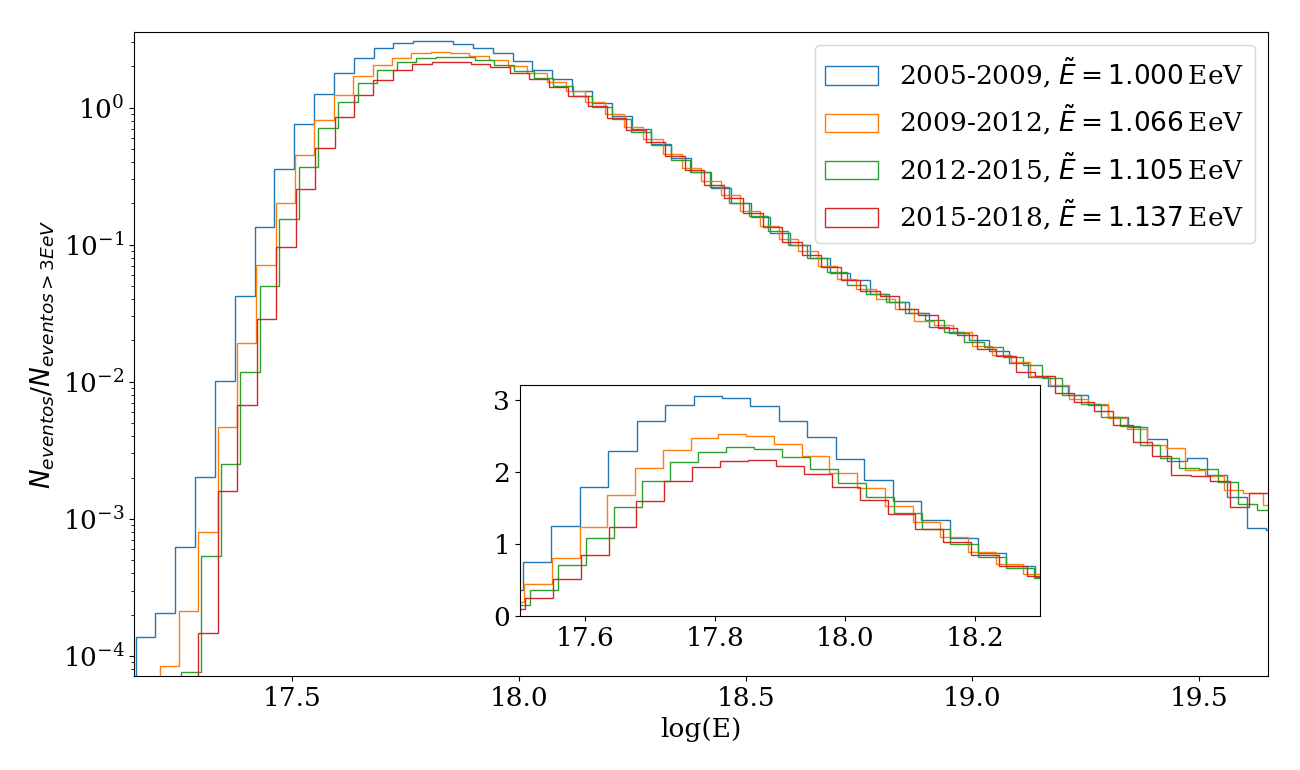
\includegraphics[width=0.75\textwidth]{histograma_evolucion_eventos.png}
	\caption{Histograma de eventos por rango de tiempo medido por el Observatorio Pierre Auger}
	\label{fig:futuro}
\end{figure}


El análisis del trabajo anterior fue realizado sobre los eventos medidos utilizando el disparo estándar del arreglo principal, cuya eficiencia varía con la energía del CR. Para el disparo estándar, los eventos con energía mayor a $3\,$EeV y $\theta_{max}<60^o$ o  por encima de $4\,$EeV y $\theta_{max}<80^o$, son detectados con una eficiencia del 100\%. Por lo tanto, el análisis de anisotropías en el rango de energía entre $1\,$EeV - $2\,$EeV, se requieren factores relacionados a la eficiencia del disparo en función de la energía. Estos factores son obtenidos de manera fenomenológica \cite{taborda}. 

Para superar esta dificultad y para poder recuperar la sensibilidad para bajas energías, a partir del año 2013  se implementó otros algoritmos de disparo en los SDs, llamados ToTd y MoPS \cite{pierre2013plans}. Estos algoritmos de disparo se mencionan en este trabajo como \textit{todos los disparos}. Con esta mejora, la eficiencia completa se alcanza a partir de una energía mayor a $1\,$EeV. De tal manera que, al estudiar los eventos en el rango $1\,$EeV - $2\,$EeV,  no son necesarios los factores de eficiencia y sólo pueden afectar los cambios de la exposición del observatorio.

Una desventaja de todos los disparos sobre el disparo estándar, es que el último tiene una mayor cantidad de eventos en el rango $1\,$EeV - $2\,$EeV, ya que se adquieren datos  desde el año 2004 con ese algoritmo. Por lo que el análisis de anisotropía con todos los disparos solo es posible desde el año 2013. 




\section{Acerca de los eventos} \label{filtro}

Se aplican cortes a los eventos para asegurar la eficiencia completa de los detectores. Estos cortes implican límites en ángulo cenital $\theta$ de los eventos, en la cantidad de vecinos al tanque de mayor señal, además de restringirse a eventos medidos en condiciones normales, es decir, cuando los sistemas de comunicación del Observatorio funciona sin inconvenientes. De esta manera, podemos prescindir de otros factores de corrección.

A partir de los registros de eventos del arreglo principal con todos los disparos, se consideran solamente los eventos que cumplan las siguientes características:

    \begin{enumerate}
      \item Ángulo cenital $\theta < 60^o$
      \item Los datos del evento son recopilados sin inconvenientes. Este filtro se conoce como \emph{Bad period flag} o $ib$. Un valor de 1 indica un buen periodo.
      \item Buena reconstrucción de la lluvia atmosférica asociada al evento.
      \item La cantidad de vecinos alrededor del tanque con mayor señal sea de 6 tanques, es decir, que el tanque de mayor señal este en el interior de un hexágono de tanques activos. Estos eventos se conocen como \textit{eventos 6T5}.
    \end{enumerate}


\section{Acerca del registro de hexágonos}\label{hexagonos_rate}

La cantidad distribución de los hexágonos activos sobre el observatorio está relacionado con el filtro de eventos $6T5$, que garantiza la calidad de la reconstrucción del evento. El observatorio lleva un registro de la cantidad de hexágonos activos cada 5 min, además de registrar las condiciones atmosféricas en distintas estaciones de clima sobre la superficie del observatorio. 

